\documentclass[xelatex,ja=standard,jafont=noto]{bxjsarticle}
\usepackage[utf8]{inputenc}

\date{May 2020}

\usepackage{natbib}
\usepackage{graphicx}
\usepackage{tikz}
\usepackage{circuitikz}
\usepackage{tabularx}
\usepackage{diagbox}
\usepackage{amsmath,amssymb}




\begin{document}



	\begin{titlepage}
			\begin{center}
				
				{\Large 令和2年}
				
				\vspace{10truept}
				
				{\Large 機械工学実験1}
				
				\vspace*{140truept}
				
				{\Huge デジタル回路アフタレポート} 
				
				\vspace{160truept}
				
				{\Large 指導教員}
				
				\vspace{10truept}
				
				{\Large yoshitaka adachi}
				
				\vspace{70truept}
				
				{\Large 芝浦工業大学}
				
				\vspace{10truept}
				
				{\Large 機械制御システム}
				
				\vspace{30truept}
				
				{\Large bq18026 関宇}      
				
			\end{center}
		\end{titlepage}








\section{課題1}
MIL 記号を用いて全加算器の回路図を描きなさい.その回路図を 74 シリーズの IC で製作する
場合の実態配線図を描きなさい.実態配線図の例を図 1 に示す.\\

全加算器は二つの半加算器とORゲートの組み合わせで構成されている。入力が三つがあり、演算される二つの二進数と下の桁からの桁上りである。Exclusive ORによる表現にを図のようになる。
		

\begin{figure}[h!]
    \centering
    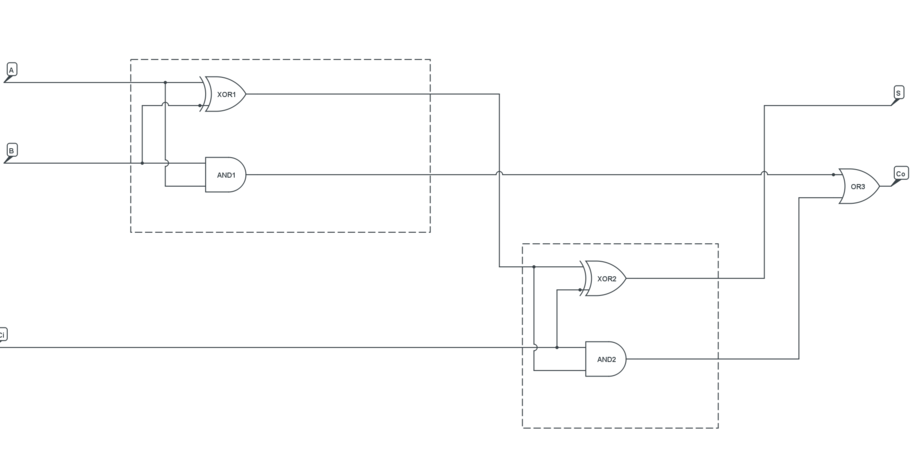
\includegraphics[scale=0.4]{xor.png}
    \caption{Exclusive ORによる表現}
\end{figure}

しかしその回路図を74シリーズのICで製作するので、つまりANDゲート、ORゲート、NOTゲートの組み合わせである。


\begin{figure}[h!]
    \centering
    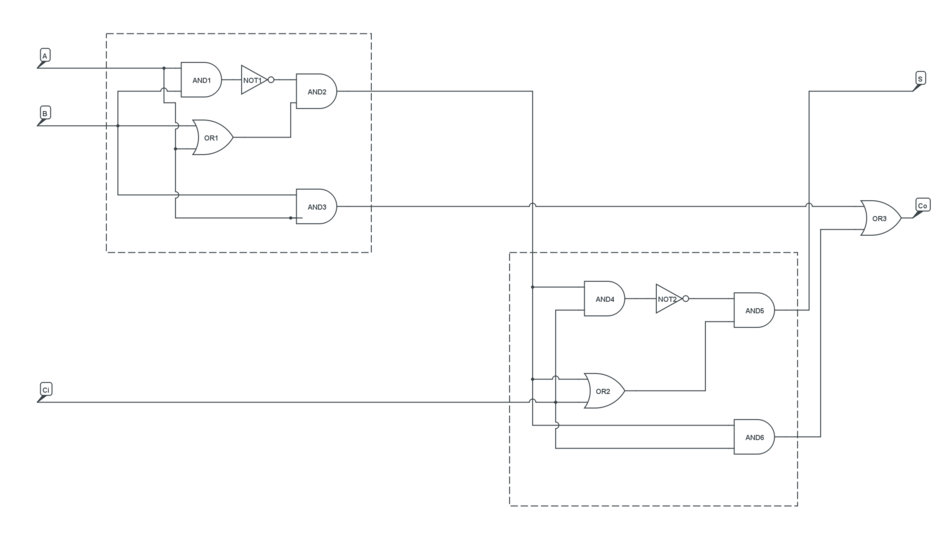
\includegraphics[scale=0.4]{fuller.png}
    \caption{全加算器}
\end{figure}



\newpage






ICの配線がICの分布によって違うので、まずICの数を考える。図面2によると、ANDゲートが6個、ORゲートが3個、NOTゲートが2個必要である。つまり7408二枚、7432、7404各一枚が必要である。\\


\begin{figure}[h!]
    \centering
    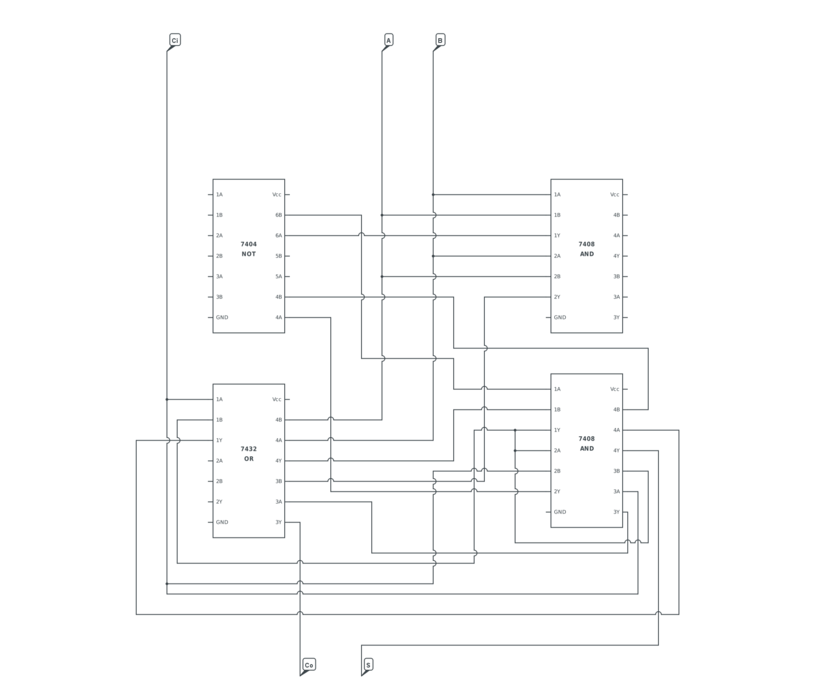
\includegraphics[scale=0.75]{IC.png}
    \caption{IC配線図}
\end{figure}




\newpage


あるいはNANDゲートによる表現もできる。


\begin{figure}[h!]
    \centering
    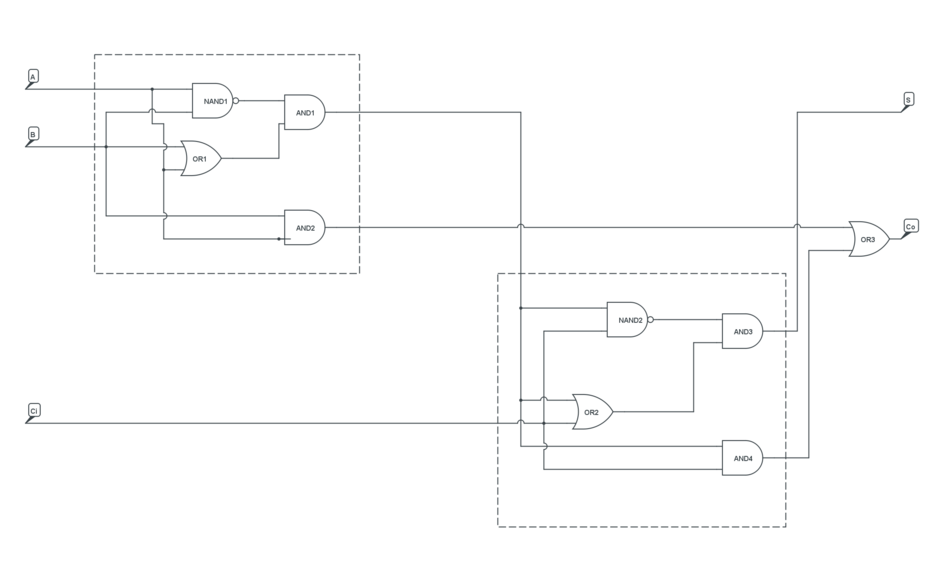
\includegraphics[scale=0.4]{nand.png}
    \caption{NANDゲートによる表現}
\end{figure}


\begin{figure}[h!]
    \centering
    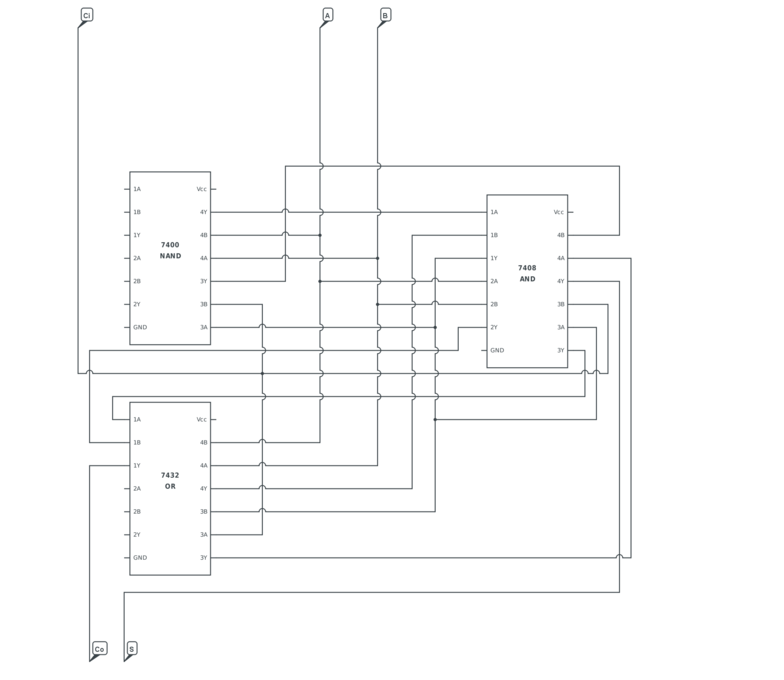
\includegraphics[scale=0.8]{nandic.png}
    \caption{NANDゲートによる配線}
\end{figure}



\section{課題2}
7404 と 7400 を使ったパルス波の発生回路を,図 2 のような TC74HC123 を使用したパルス波
発生回路に変更する.実験で計測したパルス幅に対して± 5$  \% $以内のパルス幅を発生させるために
は,TC74HC123 に接続する抵抗 R1 とコンデンサ C1 の値はいくつになるか,データシートを参
照して計算すること.抵抗とコンデンサは市販されている下記の製品を使用すること. 抵抗とコ
ンデンサは複数使用してもよい.\\

実験で計測したパルス幅は2.1$ \mu $sに対して± 5$  \%  $なのは、できて欲しいパルス幅は2$  \sim $2.2($ \mu $s)である。\\

次に、TC74HC123のデータシートより、外部抵抗R$ _{X} $はV$ _{cc} $ $ \geqq $3.0Vの時1k $ \Omega $以上の抵抗が選定することができるので、今回2k $ \Omega $の抵抗を選定する。さらにパルス幅の計算式

\begin{equation}
		t_{w}(out)\simeq 1.0C_{X}R_{X}
\end{equation}

より、コンデンサの計算ができる。結果より、1000pFのコンデンサを選定する。


\section{参考文献}

CPUをつくろう!(https://userweb.alles.or.jp/chunichidenko/mycpu140.html)

\end{document}
